\begin{savequote}[45mm]
\ascii{Any fool can write code that a computer can understand. Good programmers write code that humans can understand.}
\qauthor{\ascii{- Martin Flower}}
\end{savequote}

\chapter{原理与概念} 
\label{ch:bazel-concept}

\section{基本概念}

\begin{content}

\subsection{领域模型}

\ascii{Bazel}的核心领域模型非常简单,如\refig{bazel-domain-model}所示。\ascii{Workspace}包含零个或多个\ascii{Package},每个\ascii{Package}包括零个或多个\ascii{Target},\ascii{Target}包括\ascii{File, Rule, PackageGroup}。
 
\begin{figure}[H]
\centering
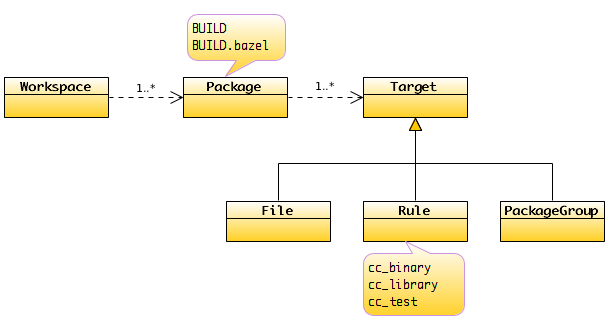
\includegraphics[width=0.9\textwidth]{figures/bazel-domain-model.png}
\caption{领域模型}
 \label{fig:bazel-domain-model}
\end{figure}

\subsection{工作区(Workspace)}

一般地,在项目的\emph{根目录}创建一个\ascii{WORKSPACE}文件,\ascii{Bazel}据此在构建过程中创建一个\emph{工作区}(\ascii{Workspace}),用于标识该项目的起始位置。在工作区内,项目所包含的所有文件,包括待构建的源文件、构建过程中自动生成的文件,及其所有外部依赖都归属于该\emph{工作区}。其中,\ascii{WORKSPACE}文件用于声明本项目的外部依赖;如果项目不存在外部依赖,\ascii{WORKSPACE}的内容可为空。

\subsubsection{隔离环境}

工作区为项目构建提供了一个安全的隔离环境。例如,本地存在两个待构建的\cpp{}项目\ascii{A}和\ascii{B},它们都依赖于第三方\cpp{}库\ascii{D}。不幸的是,它们分别依赖了不同的版本实现\ascii{v1}和\ascii{v2}。如\refig{bazel-concept-conflict}所示,问题变得非常棘手,系统目录\ascii{/usr/local/include, /usr/local/lib}应该放\ascii{D}的哪个版本呢?

\begin{figure}[H]
\centering
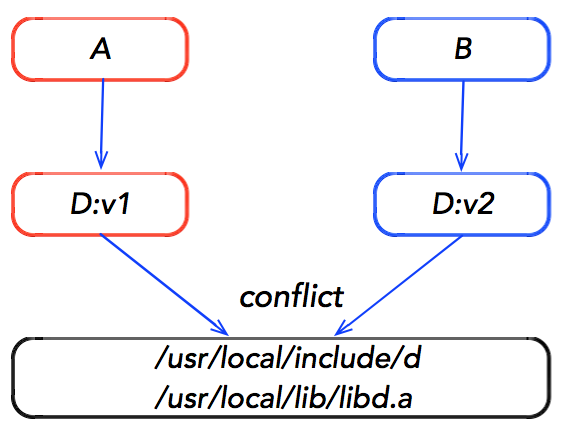
\includegraphics[width=0.5\textwidth]{figures/bazel-concept-conflict.png}
\caption{工作区:隔离构建环境}
 \label{fig:bazel-concept-conflict}
\end{figure}


归功于\ascii{Bazel}良好的隔离性,每个项目的工作区都是独立的,它们将所有依赖控制在各自的工作区,避免了第三方库的名字和版本冲突。如\refig{bazel-concept-workspace}所示。

\begin{figure}[H]
\centering
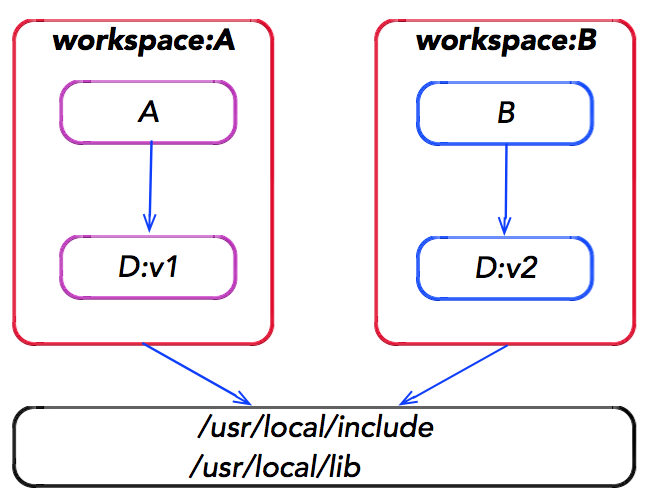
\includegraphics[width=0.5\textwidth]{figures/bazel-concept-workspace.png}
\caption{工作区:隔离构建环境}
 \label{fig:bazel-concept-workspace}
\end{figure}

\subsubsection{惯例优于配置}

按照\ascii{Bazel}的惯例,在项目根目录同时创建一个与项目名称同名的文件夹,以此定义项目命名空间的起始位置。如\refig{bazel-concept-polyflow}所示,项目名称为\ascii{polyflow},在根目录中创建文件\ascii{WORKSPACE},及其同名的子目录\ascii{polyflow};然后在子目录\ascii{polyflow}中,根据系统架构将其分解为两个基本的模块\ascii{core, util}。

\begin{figure}[H]
\centering
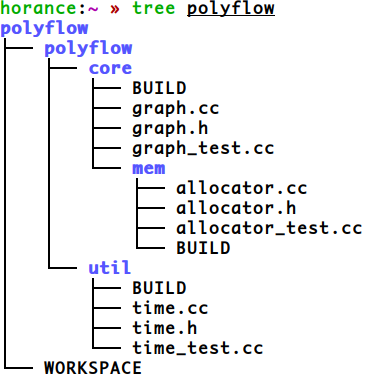
\includegraphics[width=0.6\textwidth]{figures/bazel-concept-polyflow.png}
\caption{Bazel项目组织}
 \label{fig:bazel-concept-polyflow}
\end{figure}

\subsection{包(Package)}

含有\ascii{BUILD}或\ascii{BUILD.bazel}文件的目录,\ascii{Bazel}在构建时将其标识为\emph{包}(\ascii{Package})。如果一个目录不包含\ascii{BUILD}或\ascii{BUILD.bazel}文件,则它只是一个纯粹的目录,隶属于最近的父包(\ascii{BUILD}或\ascii{BUILD.bazel}文件)。

\subsubsection{包名}

包名始于\ascii{WORKSPACE}所在的目录,由路径名组成。例如\ascii{app/core, app/core/mem}\footnote{注意,\ascii{Unix}路径名\ascii{./app/core}与包名\ascii{app/core}不等价,它们之间存在微妙的差异。}。特殊地(常见于遗留系统中),如果\ascii{BUILD}文件与\ascii{WORKSPACE}都在根目录中,此时包名为空,而不是一个点号\footnote{在\ascii{Unix}中,点号表示当前目录。},如\refig{bazel-concept-nil-package}所示。

\begin{figure}[H]
\centering
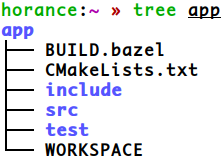
\includegraphics[width=0.35\textwidth]{figures/bazel-concept-nil-package.png}
\caption{包名为空}
 \label{fig:bazel-concept-nil-package}
\end{figure}

\subsubsection{子包}

在一个包中,递归地包含该目录下的所有文件。但是,如果某个子目录自身包含\ascii{BUILD}文件,则独立成为一个子包,并不隶属于上一级的父包。也就是说,子包独立于父包,父包不包括子包。

如\refig{bazel-concept-subpackage}所示,包\ascii{app/core}不包括包\ascii{app/core/mem},它们相互独立。但是,习惯依然称\ascii{app/core/mem}为\ascii{app/core}的子包。

\begin{figure}[H]
\centering
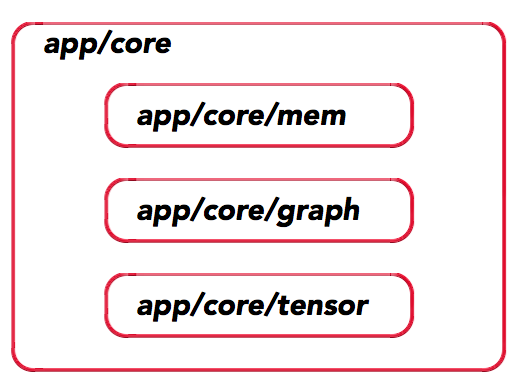
\includegraphics[width=0.4\textwidth]{figures/bazel-concept-subpackage.png}
\caption{子包}
 \label{fig:bazel-concept-subpackage}
\end{figure}



\subsection{目标(Target)}

在一个包(\ascii{Package})中,可以包含零个或多个\emph{目标}(\ascii{Target})。一般地,目标包括\emph{文件}(\ascii{File}),\emph{规则}(\ascii{Rule}),\emph{包集合}(\ascii{Package Group})三种基本类型。

\subsubsection{文件}

文件包括\emph{源文件}和\emph{派生文件}两种基本类型。例如,程序员实现的\cpp{}头文件和实现文件则称为源文件,而由\ascii{protoc}自动生成的\cpp{}头文件和实现文件则称为派生文件。

\subsubsection{规则}

在\ascii{BUILD}文件中,可以定义零个或多个\emph{规则}(\ascii{Rule})。规则由输入、输出、动作三元祖构成。因为\ascii{Bazel}使用声明式的表达方式,规则的动作往往是隐式的。例如,使用规则\ascii{cc\_library}时,无需显式地实现\ascii{g++ a.cc -o a.o}。

规则输入的文件,可能是源文件,也可以是其他规则生成的派生文件,常通过\ascii{srcs, hdrs}等属性表示。但是,规则输出的文件,必然是派生文件。此外,规则输出的派生文件,必然与该规则属于同一个包;但是,规则输入的源文件可以来自于其他包。

规则的输入也可以是规则,常通过\ascii{deps}属性表示。通过规则之间的依赖关系,构建了运行时的\ascii{DAG}图。一般地,依赖关系具有多种表现形式,而且与编程语言极其相关。例如,在编译时,\ascii{A}依赖于\ascii{B}的头文件;在链接时,\ascii{A}依赖于\ascii{B}的符号;在运行时,\ascii{A}依赖于\ascii{B}的数据。

\subsubsection{包集合}

包集合较为特殊,它标识一组包。它由\ascii{package\_group}定义。使用包集合,可以很方便地将某一个规则的可见性一并赋予给该包集合,使得该集合所包含的包都可以访问该规则。

\subsection{标签(Label)}

每个\emph{目标}都存在一个全局的名称,称为标签(\ascii{Label}),由如下几个部分组成:

\begin{nodiff}{标签}
 \begin{c++}
label = "@domain//package_name:target_name"
 \end{c++}
\end{nodiff}

其中,\ascii{@domain}, \ascii{//package\_name}, 冒号,\ascii{target\_name}在一些特殊场景下都可省略。例如,在本工作区内,完全可略去\ascii{@domain};但是,如果引用外部依赖的标签,\ascii{@domain}则是必须的。而在同一个包内,也可完全略去\ascii{//package\_name},甚至略去冒号;按照惯例,规则保留冒号,文件略去冒号。

例如,在\ascii{cub/base/BUILD}中定义了一个\ascii{placement}的基础类库,基本覆盖了所有形态的标签格式。

\begin{nodiff}{标签样例://cub/base/BUILD}
 \begin{python}
package(
    default_visibility = [    
        "//visibility:public",    
    ],
)

cc_library(
    name = "placement",
    hdrs = ["placement.h"],
)

cc_test(
    name = "placement_test",
    srcs = ["placement_test.cc"],
    deps = [ 
        ":placement",
        "//cub/algo:loop",
        "//cub/dci",      
        "@xunit_cut//:cut",
        "@xunit_cut//:cut_main",
    ],  
)
 \end{python}
\end{nodiff}

\subsubsection{文件标签}

在规则\ascii{placement\_test}的\ascii{srcs}属性定义中,标签\ascii{placement\_test.cc}略去了域名和包名,及其可选的冒号。也就是说,在\ascii{//cub/base/BUILD}中,如下标签是等价的。

\begin{nodiff}{//cub/base/BUILD}
 \begin{python}
//cub/base:placement_test.cc
:placement_test.cc # 推荐
placement_test.cc
 \end{python}
\end{nodiff}

\subsubsection{规则标签}

而在规则\ascii{placement\_test}的\ascii{deps}属性定义中,标签\ascii{:placement}略去了域名和包名,但保留了冒号,用于显式地标识它是一个规则。也就是说,在\ascii{//cub/base/BUILD}中,如下标签是等价的。

\begin{nodiff}{//cub/base/BUILD}
 \begin{python}
//cub/base:placement
:placement  # 推荐
placement
 \end{python}
\end{nodiff}

但是,标签\ascii{//cub/algo:loop}来自于另一个包\ascii{cub/algo},所以需要显式地给出全路径。

\subsubsection{同名标签}

特殊地,标签\ascii{//cub/dci}等价于\ascii{//cub/dci:dci}。也就是说,当\ascii{target\_name}等于其目录名,则常常略去\ascii{target\_name}。其中,标签\ascii{//cub/dci:dci}定义如下。

\begin{nodiff}{//cub/dci/BUILD}
 \begin{python}
package(
    default_visibility = [    
        "//visibility:public",    
    ],
)

cc_library(
    name = "dci",
    hdrs = ["role.h"],
)
 \end{python}
\end{nodiff}

注意,标签\ascii{//cub/dci}切忌不可略去\ascii{//},标签名以\ascii{//}开头,而\ascii{cub/dci}仅仅为包名。在同一个\ascii{//cub/dci/BUILD}文件中,如下标签都是等价的。

\begin{nodiff}{//cub/dci/BUILD}
 \begin{python}
//cub/dci:dci
//cub/dci
:dci
dci
 \end{python}
\end{nodiff}

\subsubsection{外部标签}

标签\ascii{@xunit\_cut//:cut}来自于第三方库\ascii{xunit\_cut},因此需要显式地加上域名。外部依赖的名称定义于\ascii{WORKSPACE}之中。按照惯例,域名推荐使用\ascii{DNS}名称,例如\ascii{github\_horanceliu\_cut},将极大降低名字冲突的概率。

\begin{nodiff}{WORKSPACE}
 \begin{python}
http_archive(
    name = "xunit_cut",
    sha256 = "f7c2c339a5ab06dc1d16cb03b157a96e6c591f9833f5c072f56af4a8f8013b53",
    strip_prefix = "cut-master",
    urls = [
        "https://github.com/horance-liu/cut/archive/master.tar.gz",
    ],
)
 \end{python}
\end{nodiff}

其中,\ascii{sha256}的值可以通过执行如下命令得到。

\begin{nodiff}{计算SHA256值}
 \begin{python}
$ curl -L https://github.com/horance-liu/cut/archive/master.tar.gz | sha256sum
 \end{python}
\end{nodiff}

\ascii{Cub}依赖于第三方库\ascii{Cut}的关系,如\refig{bazel-concept-cub-deps-cut}所示。

\begin{figure}
\centering
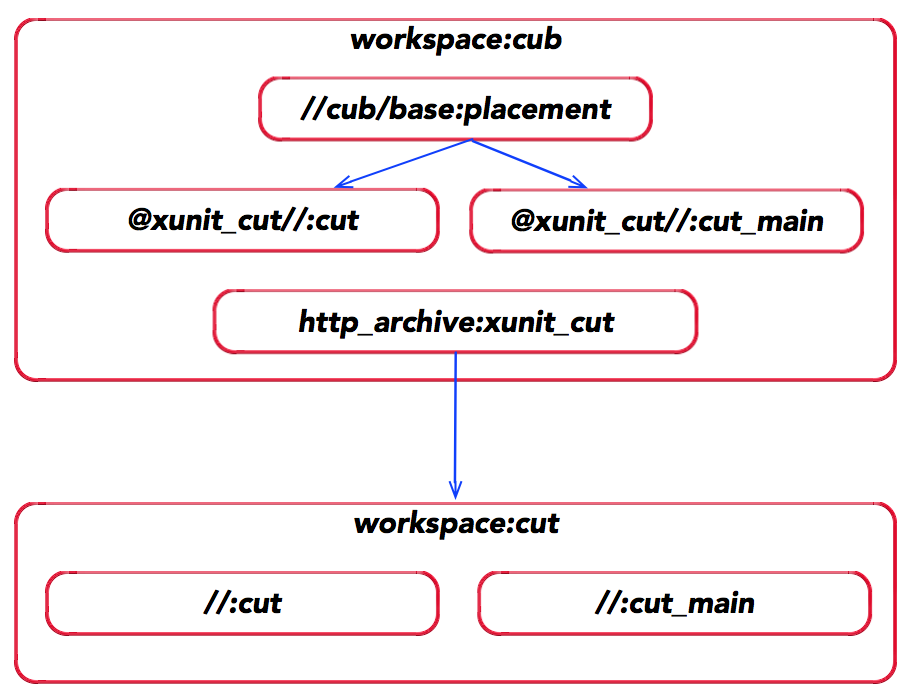
\includegraphics[width=0.8\textwidth]{figures/bazel-concept-cub-deps-cut.png}
\caption{Cub引用外部依赖Cut}
 \label{fig:bazel-concept-cub-deps-cut}
\end{figure}

\subsection{遗留系统}

\ascii{Bazel}推荐的项目组织结构,可能与遗留系统的风格存在迥异。以\ascii{Cut}为例,它原来使用\ascii{CMake}构建,并将\ascii{include, src, test}相互分离,如\refig{bazel-concept-cut}所示。

\begin{figure}[H]
\centering
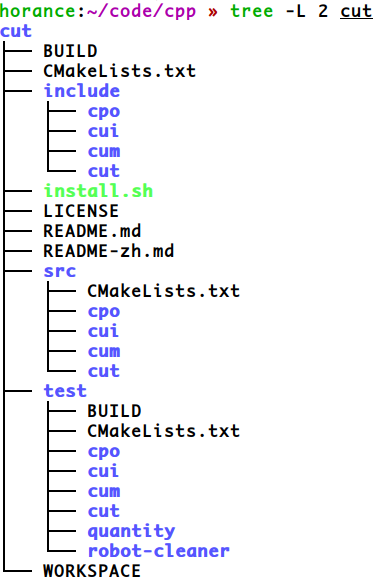
\includegraphics[width=0.6\textwidth]{figures/bazel-concept-cut.png}
\caption{GoogleTest}
 \label{fig:bazel-concept-cut}
\end{figure}

\ascii{Cut}显然违背了\ascii{Bazel}约定的惯例,但它也可以使用\ascii{Bazel}。相对于\ascii{CMake},\ascii{Bazel}的声明式表达,可读性和可维护性相当卓越。

\begin{nodiff}{Cut构建规则}
 \begin{python}
cc_library(
  name = "cut",
  srcs = glob(
      include = [ 
          "src/**/*.cc",
          "src/**/*.cpp"
      ],  
      exclude = [ 
          "src/cut/startup/main.cpp"
      ]      
  ),  
  hdrs = glob([
      "include/**/*.h", "include/**/*.hpp"
  ]), 
  copts = ["-std=c++14"],
  includes = ["include"],
  visibility = ["//visibility:public"],
)

cc_library(
  name = "cut_main",
  srcs = [ 
      "src/cut/startup/main.cpp"
  ],  
  hdrs = [ 
      "include/cut/cut.h",
      "include/cut/startup/StartUp.h",
  ],                                                                                                                        
  copts = ["-std=c++14"],
  includes = ["include"],
  visibility = ["//visibility:public"],
)
 \end{python}
\end{nodiff}

执行如下命令,启动构建\ascii{Cut}。注意,\ascii{BUILD}文件与\ascii{WORKSPACE}在同一目录,标签\ascii{//:cut\_main}的包名为空。

\begin{nodiff}{构建GoogleTest}
 \begin{python}
$ bazel build //:cut_main
 \end{python}
\end{nodiff}

\end{content}
